\documentclass[../projekt.tex]{subfiles}
\begin{document}

\chapter{Systém Fitcrack}\label{Fitcrack}
Fitcrack je systém, ktorý slúži na obnovu hesiel. Vďaka tomu že ide o~distribuovaný systém, je možné rozdelovať prácu na predom neobmedzený počet staníc, ktoré môžu byť rozmiestnené po celom svete. Je tvorený  architektúrou klient-server. Serverová časť sa stará o~prerozdeľovanie úloh medzi klientov. Klienti pracujú na výpočte kryptografických hešov a svoje výsledky posielajú na server, kde sa spracujú a vyhodnotia.
\cite{fitcrackSprava}


\label{hashcat}
\section{Hashcat}
Hashcat\footnote{\url{https://hashcat.net}} je výkonný nástroj na obnovu hesiel, ktorý využíva technológiu OpenCL. Podporuje viac ako 200 typov kryptografických hešov. O~jeho rýchlostí svedčí aj to, že v~rokoch 2010, 2012, 2014 a 2015, tím, pozostávajúci z~členov vývojárov Hashcatu, získal prvé miesto v~súťaži \textit{Crack Me If you Can}\footnote{\url{http://contest-2010.korelogic.com/team_hashcat.html}}. Žiaľ, tento nástroj sám o~sebe nepodporuje výpočet na viacerých staniciach súčasne.


\section{BOINC}
Systém Fitcrack je postavený na voľne šíriteľnom frameworku \textit{Berkeley Open Infrastructure for Network Computing} (BOINC)\footnote{\url{https://boinc.berkeley.edu/}}. Vďaka frameworku BOINC systém Fitcrack distribuuje dielčie úlohy medzi pripojených klientov, na ktorých prebieha pokus o~nájdenia hesla pomocou nástroja Hashcat.

Systém BOINC tvorí server a klienti. Pri distribuovaní výpočetných úloh prebieha komunikácia medzi klientom a serverom prostredníctvom XML správ, ktoré sa prenášajú pomocou protokolu HTTP alebo HTTPS.
Server je hlavnou súčasťou infraštruktúry BOINC. Stará sa o~distribuovanie úloh medzi klientov a spracováva výsledky od užívateľov.
Každý klient sa periodicky dotazuje na server a žiada si novú úlohu. Po prijatí výpočetnej úlohy ju spracuje a výsledok odošle na serverom. Následne žiada o~pridelenie novej úlohy.\cite{boinccitace}


\section{Architektúra systému Fitcrack}
Ako je možné vidieť na obrázku \ref{fig:archFitcrack}, architektúra systému Fitcrack je rozdelená do niekoľkých funkčných blokov. Hlavné časti systému sú serverová a klientská.

Serverová časť systému Fitcrack beží na samostatnom stroji. Dohliada na výpočetné uzly (klientov) a má na starosti plánovanie a generovanie úloh, spracovanie výsledkov z~výpočetných uzlov a riadenie distribuovaného výpočtu. Server sa na samotnom výpočte kryptografických hešov nepodiela. Serverová časť sa dá ďalej rozdeliť na moduly. Jedným z~nich je \textit{Generator}, ktorý sa stará o~vytváranie úloh pre výpočetné uzly. Ďalším modulom je \textit{Validator}. Ten slúži na overenie syntaxe odpovedi od výpočetného uzlu. \textit{Assimilator} funguje na princípe nekonečného cyklu, ktorý periodicky kontroluje a spracováva nové výsledky. V~prípade nájdenia hesla výsledok priradí do databázy, a všetkým výpočetným uzlom pošle správu aby zanechali prácu. Nástroj \textit{XtoHashcat} slúži na extrakciu šifrovacie kľúča z~rôznych typov súborov. Modul \textit{WebAdmin} poskytuje užívateľovi prototyp grafického rozhrania na správu systému. Ostatné moduly serverovej časti sú súčasťou siete BOINC.

Klient (výpočetný uzol), po pripojení žiada od servera novú úlohu, ktorú spracuje, vyrieši\footnote{Zvyčajne sa jedná o~výpočet kryptografických hešov, ale existujú aj iné typy úloh, ktoré výpočetné uzly systému Fitcrack riešia. Napríklad meranie výkonu.}, a výsledok odošle na server. V~súčasnosti sa pridelené úlohy na klientovi riešia pomocou nástroja Hashcat (viď \ref{hashcat}), ktorý nie je potrebné inštalovať, pretože sa automaticky po pripojení uzlu odošle klientovi jeho binárna verzia. Po dokončení pridelenej úlohy si klient žiada o~ďalšiu.


\begin{figure}[h]
    \centering
    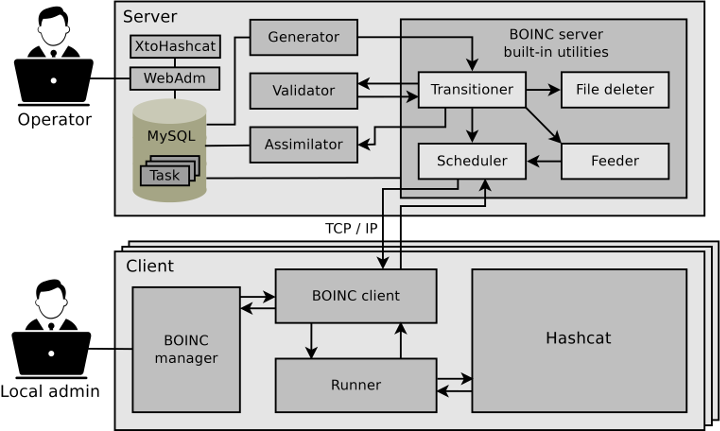
\includegraphics[scale=0.5]{obrazky/fitcrack_arch_web.png}
    \caption{Architektúra systému Fitcrack \cite{fitcrackSprava}}
    \label{fig:archFitcrack}
\end{figure}





\end{document}